\documentclass{article}[14pts]

\usepackage{graphicx}

\begin{document}

%\addtolength{\voffset}{-10mm}
%\addtolength{\hoffset}{-10mm}
%\addtolength{\topmargin}{-20mm}
%\addtolength{\textheight}{50mm}
%\addtolength{\textwidth}{20mm}

\newcommand{\phipsi}{$\phi,\psi$~}
\newcommand{\eg}{e.g.~}
\newcommand{\etc}{etc.}
\newcommand{\dfs}{\textsc{dfs}~}
\newcommand{\rapper}{\textsc{rapper}}
\newcommand{\probe}{\textsc{probe}}
\newcommand{\ie}{i.e.~}
\newcommand{\ca}{$C_\alpha$~}
\newcommand{\CA}[1]{${C_\alpha}^{#1}$~}
\newcommand{\CB}[1]{${C_\beta}^{#1}$~}
\newcommand{\C}[1]{$C^{#1}$~}
\newcommand{\N}[1]{$N^{#1}$~}
\newcommand{\cO}[1]{$O^{#1}$~}
\newcommand{\Ang}[1]{${#1}A^o$~}

\title{A flexible modular software for discrete-restraint based sampling of macromolecular conformations}

\maketitle

\section{Introduction}

this is how to cite Dunbrack's SCWRL3  \cite{scwrl3}.

Discrete, restraint based sampling of protein conformations has been shown as an effective tool in a variety of tasks that rely on conformational exploration, such as loop building, comparative modelling, solving low resolution X-ray data, building an ensemble of models to explain the X-ray density, \etc Minimization-based protocols perform better when they optimize structures calculated with this methodology. Discrete restraint-based conformational sampling does not have the problems of local minima, nor various energy terms need be reconciled. Sampled conformations are scattered uniformly on the energy landscape, thus making them a very good starting ensemble for further minimization. \rapper, a popular tool developed in our lab for sampling protein conformations, has effectively demonstrated these advantages.

It is worth applying this promising technique to a broader set of problems in structural biology. The technique should be extended to other kinds of macromolecules, including oligonucleotides and carbohydrates. It should be possible to sample conformational flexibility of interfaces in protein-protein, protein-ligand and protein-DNA complexes. It should be possible to handle ensemble-averaged restraints, \eg NOE restraints from NMR experiments. It should be possible to build coarse-grained models based on cryoEM data, followed by all-atom modeling based on X-ray data. It should be easy to incorporate knowledge-based restraints, such as conformational preferences of certain amino-acid sequences.

The main challenge in achieving these objectives is technical in nature. Extending C++ codebase (including \rapper) is not straightforward as it demands expertise and sufficient hacking time. This technical barrier makes the big idea inaccessible. A popular solution for such challenges is to adopt a hybrid, multi-layered code architecture that combines compiled and interpreted languages, retaining advantages of both. While the compiled language (\eg C++) remains at the core of the software, the interpreted language (\eg Python) provides easy access to the functionality. Good design of the core enables easy extension of the software to address related problems.

In this paper, we introduce a new tool that makes \rapper methodology more accessible and extensible. After describing the design and implementation, we compare the tool with \rapper's \CA-tracing performance and demonstrate that our tool can be a good substitute for \rapper. Then we apply the tool to new scenarios and show its versatility. We conclude by discussing future applications.

We have attempted to make the new tool as modular and flexible as possible. For this, we have chosen a python-swig-cpp style of coding, whereby interface of cpp code is exposed in python. Python is an object-oriented scripting language known for its versatility and cleanliness. Python-swig-cpp style has been used before in many well-known academic tools, \eg xplor-nih, because this style gives industrial robustness without losing the fluidity needed in academic implementations.

\section{Design}
While staying within the realm of discrete, restraint-based sampling, we aim to provide as much flexibility to the end-user as possible. This is achieved by appropriate division of tasks between compiled and interpreted languages. By default, a task is coded in interpreted language and only when necessary, the compiled language is used. We have chosen Python and C++ as our interpreted and compiled languages respectively due to their dominance in their respective language categories. SWIG is used to generate python-callable wrappers around C++ code.

Non-repititve, high level tasks in discrete restraints based modeling are model representation, assignment of atomic and covalent properties, information retrieval, parsing and persistence \etc They are best assigned to python scripts rather than C++. Repititve tasks include sampling of knowledge-based distributions, 3D coordinate calculation, hard-sphere collision detection \etc and they are well-addressed by C++ modules which are imported in Python using SWIG.

Major abstractions and concepts currently used in the software are described below. Their standardized interfaces are used by high level application script to address a specific problem.

\subsection{Pointset}
This is the set of 3D coordinates in the system under consideration, with their hard-sphere (van der Waal) radii. Some points are already known and need not be computed, \eg rest of the structure in a loop building exercise, or well-resolved portions of electron density map. A high-level application script generates the pointset. Builders and restraints operate on a group of indices in a pointset.

\subsection{Samplers}
A sampler samples an underlying distribution and returns a sampled datum. Well-known examples are \phipsi sampling for protein backbone and rotamer sampling for sidechains. New types of sampling, \eg multiple \phipsi and all those arising from knowledge-based preferences, can be easily incorporated by writing new samplers for that data, which is used for builder of that entity, say 3-residue long fragments.

\subsection{Restraints}
Values of various geometric entites are useful in constraining the conformational space, \eg distance restraints in NMR data, electron-density from X-ray data, \ca positional information derived from templates in comparative modelling, and so on. A restraint object holds the information of points on which it is to be tested, and the intelligence for testing. A restraint is generally binary, it either satisfied or violated. A restraint can be optional also, in which case it may be discarded if not satisfiable.

\subsection{Builders}
A conformation is built step-by-step in discrete restraint-based sampling, in contrast to approaches which start with a random or an intelligently guessed complete conformation. In each step, depending on atomic coordinates data at that instant, coordinates of a few more atoms are calculated. Essentially, there is a builder acting on an atomset to generate another atomset. For instance, a simple \phipsi sampling based peptide backbone builder uses coordinates of \C{i-2}, \N{i-1}, \CA{i-1} to calculate \C{i-1}, \N{i}, \CA{i} coordinates; \N{i}, \CA{i}, \CB{i} coordinates are required to find sidechain coordinates from a sample of $\chi$ angles, and so on. Thus all coordinate calculations can be represented as builders. A builder is aware of indices of it depends upon and calculates. It may also require an appropriate sampler, in which case there is a limit on number of sampling attempts for a builder. In order to avoid futile sampling, like multiply sampling the same rotamer state, builder implements a session. During a session, only new samples are used and samples already seen in that session are ignored.

\subsection{Sampling Strategy}
Sampling strategy orchestrates the restraints, samplers and builders systematically to generate conformations. Sampling strategy can be divided into ordering and execution of restraints and builders.
\subsubsection{Ordering of builders and restraints}
A correct strategy must consider builder order and builder-restraint order. There is a partial ordering induced on builders due to their input and output atomsets, \ie a builder cannot be executed unless its input atomset has been computed. Exception is builders with input atomsets consisting of known atoms, such builders are independent of other builders. Thus there is a digraph of builders, with possibly many independent builders and others depending on one or more builders. Restraints can be checked only after all atoms involved have been computed, thus giving rise to a restraint-builder dependence. An efficient strategy must test a restraint as early as possible, in order to stop sampling the disallowed region of conformational space. Once a builder succeeds or fails in its task, an efficient sampling strategy must use the builder dependece digraph to find out the builder to be attempted next. The strategy currently implemented in the tool determines the builder order by topological sort on builder digraph, more specifically as follows :
\begin{itemize}
\item In case of multiple parentless builders, a dummy builder is assumed to be their parent. A procedure similar to \dfs (depth first search) is used to assign unique parents to all nodes, \ie convert the digraph into a tree. A node appears as child of another node only if the latter is the only unvisited parent of the former.
\item Size of subtree rooted at each node is found.
\item Using \dfs again, an order is established for the nodes. When a node is popped off the \dfs stack, its children are pushed onto the stack in the ascending order of subtree sizes.
\item The order thus obtained is the final ordering used by the default strategy. If a builder fails, its unique parent builder is executed, and results of the parent and all its children are discarded. If a builder succeeds, builder next in order is called. 
\item From this order, we determine the builder immediately after which, a restraint has all the necessary points computed for checking. Thus every builder has associated restraints to check after its building task.
\end{itemize}
This will be clearer in examples worked out later. Default ordering can be easily overridden to impose an ordering of one's liking.

\subsubsection{Execution of builders and restraints}
Once the ordering among builders and restraints is established, various search strategies can be used to sample conformational space. The simplest is exhaustive search, where each restraints-satisfying option available to a builder is explored. \rapper uses a sophisticated population search algorithm, where a population of restraint-satisfying conformers is maintained at every step of build process. We have implemented both the naive and population-based search strategies. We have added a modified version of population search which backtracks a limited number of steps in case of not finding any satisfactory conformer at some step.

\subsection{Clashchecking grid}
Steric clashes are a very important restraint on conformational freedom. Hence output of every builder is verified with a 3D grid which uses geometric caching to check the clashes efficiently. In addition to pointset and associated set of hard-sphere radii, the grid accepts a list of points to be excluded from clashchecking for any point. This is useful in avoiding clashchecks with $1^{st}$ and $2^{nd}$ covalent neighbours. Reductions in sum of radii can be provided for pairs of points, so as to allow hydrogen bonding, disulphide bonding, \etc

\subsection{Application script}
Application is a high-level python script which applies the builders, restraints, samplers and sampling strategy to the problem of interest. It processes the problem inputs into a set of data structures used by the framework described here. More specifically, it creates pointset, assigns known coordinates where possible and assigns hard-sphere radii. It creates builders, samplers and restraints. It chooses a strategy and provides it a model renderer to output successfully built models, before executing the strategy.


With this design, a varierty of problems in structural biology seem addressable, because
\begin{itemize}
\item Any level of granularity can be chosen to represent the structure.
\item User need not specify the order on restraints and builders, but a preferred order may be imposed if needed.
\item Any number of coordinates may be known before modelling. They can be used as restraints or to make indepent builders.
\item Ensemble building and average restraints can be introduced easily. An ensemble strategy needs to grow a set of structures, each of which is compliant with non-ensemble restraints, and verify that this ensemble satisfies ensemble restraints too.
\item Alternate techniques can be easily introduced, \eg a sidechain rotamer library can be replaced with another by changing the builders, or a combination of many libraries can be used.
\end{itemize}

\section{Examples}

\subsection{Loop modeling}
Loop modelling is a sandbox for all modeling tools. We illustrate the execution of the tool for loop GLU (A 106) - LEU (A 112) in pdb 1f0y. The application script formulates the problem as follows:
\begin{itemize}
\item Let $start, end$ be the residues given as inputs with a pdb file.
\item \C{start-1}, \cO{start-1} in that residue are assumed unknown but are tightly restrained around their given locations within a small spheres (say \Ang{0.5} or \Ang{1}).
Similarly, \N{end+1}, \CA{end+1} are assumed as unknown in that residue, but are tightly restrained around their given locations. All mainchain and sidechain atoms in between them are modeled.
\item Similar to \rapper, van der Waal radii are taken from \probe (Richardson et al) radii with reduction factor of $0.79$, and sidechain atoms are further reduced by a factor of $0.8$.
\item \phipsi sampling is done using \rapper's \phipsi libraries.
\item Backbone dependent sidechain rotamer library (Dunbrack group) is used for sidechain sampling.
\item Peptide builders to build \CA{start} till \CA{end+1}, both included, are used. \CB{} and sidechain builders are used wherever necessary between $start-1$ and $end$, both included.
\item Depending upon covalent connectivity, clash exclusion lists are generated for all points to be modeled.
\item Spherical positional restraint, radius $3.8 * (end+1-i)$ centered on \CA{end+1}, is imposed on each \CA{i} atom in range $start, end$. Another similar restraint with radius $3.8 * (i-start+1)$ + distance(\CA{start-1},\CA{end+1}) is also imposed on \CA{i}. This restraint is generated from triangle inequality relation between \CA{i}, \CA{start-1}, \CA{end+1}.
\end{itemize}

The strategy described earlier finds digraph of builder dependencies, as shown in fig.\ref{loop-digraph}. The digraph is converted into a tree and the topological order is determined as shown in fig.\ref{loop-tree}.

% We made 100 attempts to generate loop models with this script. With \Ang{1} restraints on \N{end+1} and \CA{end+1}, k models were obtained with least, mean and worst \CA{} \rmsd of 1, 2, 3.

\begin{figure}
\includegraphics[width=6in,angle=90]{digraph.ps}
\caption{Builder dependence digraph for loop modeling.}
\label{loop-digraph}
\end{figure}

\begin{figure}
\includegraphics[width=4in]{tree.ps}
\caption{Tree obtained from digraph shows builder fallback (black edges) and topological order (red edges).}
\label{loop-tree}
\end{figure}


\section{Benchmarking}
We choose \CA{} tracing to compare the performance of this tool with \rapper, because it is a good representative of problems addressed with \rapper. It tests the capability of sampling long peptide chains under loose and tight restraints. A tool which can do \CA{} tracing satisfactoriy can be extended to trace through electron density, building missing regions in a structure and homology modeling.

\subsection{mainchain-only model accuracy as a function of CA-restraint threshold}

\subsection{modellability under strict restraints}

\subsection{all-atom model accuracy as a function of centroid restraint threshold (chi also)}

\subsection{mainchain and all-atom accuracy under random-error restraints}

\subsection{execution time to get mainchain (1A CA) and all-atom model (1A CA and 1A centroid)}

\bibliography{refs}
\bibliographystyle{bioinformatics}

\end{document}
